%%%%%%%%%%%%%%%%%%%%%%%%%%%%%%%%%%%%
% Slide options
%%%%%%%%%%%%%%%%%%%%%%%%%%%%%%%%%%%%

% Option 1: Slides with solutions

\documentclass[slidestop,compress,mathserif]{beamer}
\newcommand{\soln}[1]{\textit{#1}}
\newcommand{\solnGr}[1]{#1}
\usepackage{booktabs}

% Option 2: Handouts without solutions

%\documentclass[11pt,containsverbatim,handout]{beamer}
%\usepackage{pgfpages}
%\pgfpagesuselayout{4 on 1}[letterpaper,landscape,border shrink=5mm]
%\newcommand{\soln}[1]{ }
%\newcommand{\solnGr}{ }

%%%%%%%%%%%%%%%%%%%%%%%%%%%%%%%%%%%%
% Style
%%%%%%%%%%%%%%%%%%%%%%%%%%%%%%%%%%%%
%%%%%%%%%%%%%%%%%%%%%%%%%%%%%%%%%%%%%%%%%%%%%%%%%%%%%%%%%%%%%%%%%%%%%%%%
% MA213/214 shared slide style
%
% "Calm & Cool" palette + content-type callout boxes.
% Overhauled (2026) from the original OpenIntro/metropolis style:
%   - all OpenIntro visual branding removed (logo, grid, colors)
%   - a low-key cool palette (see colors below)
%   - tcolorbox callout boxes so students recognize content types
% See common/README.md for the command cheat-sheet.
%%%%%%%%%%%%%%%%%%%%%%%%%%%%%%%%%%%%%%%%%%%%%%%%%%%%%%%%%%%%%%%%%%%%%%%%

\usetheme{metropolis}

%%%%%%%%%%%%%%%%
% Packages
%%%%%%%%%%%%%%%%

\usepackage{geometry}
\usepackage{graphicx}
\usepackage{amssymb}
\usepackage{epstopdf}
\usepackage{amsmath}  	% this permits text in eqnarray among other benefits
\usepackage{url}		% produces hyperlinks
\usepackage{hyperref}	% allows for color usage in tables
\usepackage[english]{babel}
\usepackage[latin1]{inputenc}
\usepackage{colortbl}	% allows for color usage in tables
\usepackage{multirow}	% allows for rows that span multiple rows in tables
\usepackage{color}		% this package has a variety of color options
\usepackage{pgf}
\usepackage{calc}
\usepackage{ulem}
\usepackage{multicol}
\usepackage{textcomp}
\usepackage{txfonts}
\usepackage{listings}
\usepackage{tikz}
\usepackage{array}
\usepackage{wasysym}
\usepackage{fancyvrb}
\usepackage{etoolbox}             % \ifstrempty for optional box subtitles
\usepackage[most]{tcolorbox}      % content-type callout boxes
\tcbuselibrary{listings}          % R-code block (\begin{rblock})
\usepackage{fontawesome5}         % box icons

%%%%%%%%%%%%%%%%
% Remove navigation symbols
%%%%%%%%%%%%%%%%

\setbeamertemplate{navigation symbols}{}

%%%%%%%%%%%%%%%%
% "Calm & Cool" palette
%%%%%%%%%%%%%%%%

% chrome / structure / body
\definecolor{ccSlate}{HTML}{2E3742}   % frametitle bar, structure, section pages (deep neutral slate)
\definecolor{ccInk}{HTML}{2B2B2B}     % body text
\definecolor{ccWash}{HTML}{FCF8F1}    % gentle warm title-slide background wash (complements the cool blues)

% example (blue)
\definecolor{ccBlue}{HTML}{2F6690}
\definecolor{ccBlueBg}{HTML}{EAF1F7}
% interactive activity / discussion (green)
\definecolor{ccGreen}{HTML}{4E8A6B}
\definecolor{ccGreenBg}{HTML}{E9F3EC}
% solution (purple)
\definecolor{ccPurple}{HTML}{6F5499}
\definecolor{ccPurpleBg}{HTML}{EFEAF6}
% worksheet / focused work (terracotta)
\definecolor{ccTerra}{HTML}{C2693E}
\definecolor{ccTerraBg}{HTML}{FAEDE4}
% formula / definition (neutral slate)
\definecolor{ccGray}{HTML}{5C6B7A}
\definecolor{ccGrayBg}{HTML}{EEF1F4}
% caution / common pitfall (brick red)
\definecolor{ccRed}{HTML}{B23A48}
\definecolor{ccRedBg}{HTML}{FAEAEC}
% key idea / takeaway (muted gold)
\definecolor{ccGold}{HTML}{9C7A28}
\definecolor{ccGoldBg}{HTML}{F7F1DF}
% learning goals / lesson outcomes (teal)
\definecolor{ccTeal}{HTML}{2C6E6B}
\definecolor{ccTealBg}{HTML}{E6F0EF}
% learning objectives (indigo)
\definecolor{ccIndigo}{HTML}{45507A}
\definecolor{ccIndigoBg}{HTML}{ECEEF4}
% R code / output (gray)
\definecolor{ccCode}{HTML}{5F5E5A}
\definecolor{ccCodeBg}{HTML}{F4F5F6}

% neutral grays kept from the original style
\definecolor{gray}{rgb}{0.5, 0.5, 0.5}
\definecolor{darkGray}{rgb}{0.3, 0.3, 0.3}
\definecolor{darkerGray}{rgb}{0.2, 0.2, 0.2}

% Backwards-compatible aliases: old OpenIntro color names now point at the
% new palette, so existing \textcolor{oiB}{...}, \hl{...}, etc. keep working.
\colorlet{oiB}{ccBlue}
\colorlet{oiG}{ccGreen}
\colorlet{hlblue}{ccBlue}
\colorlet{rubineRed}{ccRed}
\colorlet{irishGreen}{ccGreen}
\colorlet{lightGreen}{ccGreen}

%%%%%%%%%%%%%%%%
% Restyle metropolis with the Calm & Cool chrome
%%%%%%%%%%%%%%%%

\metroset{block=fill}

\setbeamercolor{normal text}{fg=ccInk, bg=white}
\setbeamercolor{structure}{fg=ccSlate}
\setbeamercolor{alerted text}{fg=ccBlue}
\setbeamercolor{example text}{fg=ccGreen}
\setbeamercolor{frametitle}{bg=ccSlate, fg=white}
\setbeamercolor{progress bar}{fg=ccBlue}
\setbeamercolor{title separator}{fg=ccBlue}
\setbeamercolor{title}{fg=ccSlate}
\setbeamercolor{subtitle}{fg=ccBlue}
\setbeamercolor{author}{fg=ccInk}
\setbeamercolor{institute}{fg=ccGray}
\setbeamercolor{date}{fg=ccGray}
\setbeamercolor{section title}{fg=ccSlate}
\setbeamercolor{standout}{fg=white, bg=ccSlate}

% Section pages sit on the same warm wash as the title slide. We keep
% metropolis's section-title styling and just paint a full-page ccWash
% background behind it (needs >=2 pdflatex passes for the current-page node).
\setbeamertemplate{section page}{%
  \begin{tikzpicture}[remember picture, overlay]
    \fill[ccWash] (current page.south west) rectangle (current page.north east);
  \end{tikzpicture}%
  \centering
  \begin{minipage}{22em}
    \raggedright
    \usebeamercolor[fg]{section title}%
    \usebeamerfont{section title}%
    \insertsectionhead\\[-1ex]
    \usebeamertemplate*{progress bar in section page}%
    \par
  \end{minipage}\par
  \vspace{\baselineskip}
}

%%%%%%%%%%%%%%%%
% Custom inline text commands (recolored to the palette)
%%%%%%%%%%%%%%%%

% degree
\newcommand{\degree}{\ensuremath{^\circ}}

% cite
\newcommand{\ct}[1]{
\vfill
{\tiny #1}}

\newcommand{\NamedNote}[2]{
\rule{2.5cm}{0.25pt} \\ \textit{\footnotesize{\textcolor{rubineRed}{#1:} \textcolor{darkerGray}{#2}}}}

% Note
\newcommand{\Note}[1]{
\rule{2.5cm}{0.25pt} \\ \textit{\footnotesize{\textcolor{rubineRed}{Note:} \textcolor{darkerGray}{#1}}}}

% Remember
\newcommand{\Remember}[1]{\textit{\scriptsize{\textcolor{ccTerra}{Remember:} #1}}}

% expected counts
\newcommand{\ex}[1]{\textit{\textcolor{ccBlue}{#1}}}

% red
\newcommand{\red}[1]{\textit{\textcolor{rubineRed}{#1}}}

% pink
\newcommand{\pink}[1]{\textit{\textcolor{rubineRed!90!white!50}{#1}}}

% green
\newcommand{\green}[1]{\textit{\textcolor{irishGreen}{#1}}}

% orange
\newcommand{\orange}[1]{\textit{\textcolor{ccTerra}{#1}}}

% links: webURL, webLink, appLink
\newcommand{\webURL}[1]{\urlstyle{same}{ \textit{\textcolor{darkGray}{\url{#1}}}}}
\newcommand{\webLink}[2]{\href{#1}{\textcolor{darkGray}{{#2}}}}
\newcommand{\appLink}[2]{\href{#1}{\textcolor{white}{{#2}}}}

% mail
\newcommand{\mail}[1]{\href{mailto:#1}{\textit{\textcolor{darkGray}{#1}}}}

% highlighting: hl, hlGr, mathhl
\newcommand{\hl}[1]{\textit{\textcolor{hlblue}{#1}}}
\newcommand{\hlGr}[1]{\textit{\textcolor{lightGreen}{#1}}}
\newcommand{\mathhl}[1]{\textcolor{hlblue}{\ensuremath{#1}}}

%%%%%%%%%%%%%%%%
% Structural helpers (unchanged from the original)
%%%%%%%%%%%%%%%%

% two col: two columns
\newenvironment{twocol}[4]{
\begin{columns}[c]
\column{#1\textwidth}
#3
\column{#2\textwidth}
#4
\end{columns}
}

% slot (for probability calculations)
\newenvironment{slot}[2]{
\begin{array}{c}
\underline{#1} \\
#2
\end{array}
}

% pr: left and right parentheses
\newcommand{\pr}[1]{
\left( #1 \right)
}

% cancel
\newcommand{\cancel}[1]{%
    \tikz[baseline=(tocancel.base)]{
        \node[inner sep=0pt,outer sep=0pt] (tocancel) {#1};
        \draw[red, line width=0.5mm] (tocancel.south west) -- (tocancel.north east);
    }%
}

% removepagenumbers
\newcommand{\removepagenumbers}{%
  \setbeamertemplate{footline}{}
}

% change margin
\newenvironment{changemargin}[2]{%
\begin{list}{}{%
\setlength{\topsep}{0pt}%
\setlength{\leftmargin}{#1}%
\setlength{\rightmargin}{#2}%
\setlength{\listparindent}{\parindent}%
\setlength{\itemindent}{\parindent}%
\setlength{\parsep}{\parskip}%
}%
\item}{\end{list}}

% footnote
\long\def\symbolfootnote[#1]#2{\begingroup%
\def\thefootnote{\fnsymbol{footnote}}\footnote[#1]{#2}\endgroup}

% commands from the book
\newenvironment{data}[1]{\texttt{#1}}{}
\newenvironment{var}[1]{\texttt{#1}}{}
\newenvironment{resp}[1]{\texttt{#1}}{}

%%%%%%%%%%%%%%%%
% Content-type callout boxes (tcolorbox)
%
% Each type has a colored title strip (icon + label) over a light fill.
% Color = content type; the label + icon reinforce it (so the cue does
% not rely on color alone).
%%%%%%%%%%%%%%%%

\tcbset{
  cccallout/.style 2 args={
    enhanced, breakable=false,
    colback=#2, colframe=#1, colbacktitle=#1, coltitle=white,
    fonttitle=\bfseries\footnotesize,
    boxrule=0.6pt, arc=2.5pt, outer arc=2.5pt,
    left=5pt, right=5pt, top=3pt, bottom=3pt, boxsep=2pt,
    toptitle=2pt, bottomtitle=2pt, lefttitle=5pt,
    before skip=5pt, after skip=5pt,
  },
}

% One-off / collection of examples (blue): \workedexample[subtitle]{body}.
% (Named \workedexample, not \example, because beamer defines \example.)
\newtcolorbox{examplebox}[1][]{cccallout={ccBlue}{ccBlueBg},
  title={\faIcon{lightbulb}~~Example\ifstrempty{#1}{}{ \textmd{---}\ #1}}}
\newcommand{\workedexample}[2][]{\begin{examplebox}[#1]#2\end{examplebox}}

% Running-example header (blue): \examplehead{name} at the top of each frame of a
% multi-slide running example. A one-off or a collection of examples uses the
% \workedexample box above instead.
\newcommand{\examplehead}[1]{%
  \vspace{-0.4em}\par\noindent\tcbox[on line, colback=ccBlue, colframe=ccBlue, coltext=white,
    boxrule=0pt, arc=2pt, left=5pt, right=5pt, top=1pt, bottom=1pt,
    box align=base, nobeforeafter]{\footnotesize\bfseries\faIcon{lightbulb}\,Running example}%
  \ifstrempty{#1}{}{\enspace{\footnotesize\bfseries\textcolor{ccBlue}{#1}}}%
  \par\nobreak\vspace{-0.6em}{\color{ccBlue}\rule{\linewidth}{0.7pt}}\par\nobreak\vspace{-0.8em}}

% Interactive activity (green): \activity[subtitle]{body}
\newtcolorbox{activitybox}[1][]{cccallout={ccGreen}{ccGreenBg},
  title={\faIcon{users}~~Activity\ifstrempty{#1}{}{ #1}}}
\newcommand{\activity}[2][]{\begin{activitybox}[#1]#2\end{activitybox}}

% Discussion question (green): \dq{body}
\newtcolorbox{dqbox}{cccallout={ccGreen}{ccGreenBg}, title={\faIcon{comments}~~Discussion}}
\newcommand{\dq}[1]{\begin{dqbox}#1\end{dqbox}}

% Solution (purple): \solnbox{body}. Gated by the per-deck \soln toggle, so it
% shows in the instructor build and vanishes from the student handout build.
% (Named \solnbox, not \solution, because beamer already defines \solution.)
\newtcolorbox{solutionbox}{cccallout={ccPurple}{ccPurpleBg}, title={\faIcon{key}~~Solution}}
\newcommand{\solnbox}[1]{\soln{\begin{solutionbox}#1\end{solutionbox}}}

% Worksheet / focused work (terracotta): \worksheet[subtitle]{body}
\newtcolorbox{worksheetbox}[1][]{cccallout={ccTerra}{ccTerraBg},
  title={\faIcon{pencil-alt}~~Worksheet\ifstrempty{#1}{}{ #1}}}
\newcommand{\worksheet}[2][]{\begin{worksheetbox}[#1]#2\end{worksheetbox}}

% Formula / definition (neutral slate). Supports both real usages found in the
% decks: \formula{title}{body} and the bare \formula{body} (title defaults to
% "Formula"). The second group is an optional brace argument.
\newtcolorbox{formulabox}[1][Formula]{cccallout={ccGray}{ccGrayBg},
  title={\faIcon{square-root-alt}~~#1}}
\NewDocumentCommand{\formula}{m g}{%
  \IfNoValueTF{#2}%
    {\begin{formulabox}#1\end{formulabox}}%
    {\begin{formulabox}[#1]#2\end{formulabox}}}

% Common pitfall / caution (brick red): \caution[subtitle]{body}
\newtcolorbox{cautionbox}[1][]{cccallout={ccRed}{ccRedBg},
  title={\faIcon{exclamation-triangle}~~Caution\ifstrempty{#1}{}{ #1}}}
\newcommand{\caution}[2][]{\begin{cautionbox}[#1]#2\end{cautionbox}}

% Key idea / takeaway (muted gold): \keyidea[subtitle]{body}
\newtcolorbox{keyideabox}[1][]{cccallout={ccGold}{ccGoldBg},
  title={\faIcon{star}~~Key idea\ifstrempty{#1}{}{ #1}}}
\newcommand{\keyidea}[2][]{\begin{keyideabox}[#1]#2\end{keyideabox}}

% Learning goals / lesson outcomes (teal): \goals{body}. Sits under the short
% LO headings on the objectives slide; body is the "you should be able to" list.
\newtcolorbox{goalsbox}{cccallout={ccTeal}{ccTealBg}, fontupper=\footnotesize,
  top=1pt, bottom=2pt, boxsep=1pt, before skip=3pt,
  title={\faIcon{bullseye}~~By the end of today, you should be able to\ldots}}
\newcommand{\goals}[1]{\begin{goalsbox}#1\end{goalsbox}}

% Learning objectives (indigo): \objectives{body} -- the formal LO headings,
% shown alongside \goals on the objectives slide.
\newtcolorbox{objectivesbox}{cccallout={ccIndigo}{ccIndigoBg}, fontupper=\small,
  top=1pt, bottom=2pt, boxsep=1pt, before skip=3pt,
  title={\faIcon{clipboard-list}~~Learning objectives}}
\newcommand{\objectives}[1]{\begin{objectivesbox}#1\end{objectivesbox}}

% Defaults for a bare \begin{lstlisting}. Without these it inherits the listings
% package defaults: 11pt type, fixed-width columns (which spaces code out as
% "a g e _ f i t"), and no line breaking, so a long line silently runs off the
% right edge of the slide. A deck that passes its own basicstyle still wins.
% Layout only -- syntax coloring is left to the \begin{rblock} environment.
\lstset{
  basicstyle=\ttfamily\footnotesize, columns=fullflexible,
  breaklines=true, breakindent=1.5em, showstringspaces=false,
  numbers=none, frame=none}

% R code / output (gray): \begin{rblock}[subtitle] ... \end{rblock}
% NOTE: a frame containing an rblock must be declared \begin{frame}[fragile].
\lstdefinestyle{ccR}{
  language=R, basicstyle=\ttfamily\footnotesize, columns=fullflexible,
  breaklines=true, showstringspaces=false, numbers=none, frame=none,
  keywordstyle=\color{ccBlue}, commentstyle=\color{ccGreen!75!black},
  stringstyle=\color{ccTerra}}
\newtcblisting{rblock}[1][]{cccallout={ccCode}{ccCodeBg},
  title={\faIcon{terminal}~~R\ifstrempty{#1}{}{ #1}},
  listing only, listing style=ccR}

% --- Legacy boxes (kept so existing decks compile) ---

% app: application exercise -> alias of activity
\newcommand{\app}[1]{\activity{#1}}

% pq: practice question (green, interactive family)
\newtcolorbox{pqbox}{cccallout={ccGreen}{ccGreenBg}, title={\faIcon{list-ol}~~Practice}}
\newcommand{\pq}[1]{\begin{pqbox}#1\end{pqbox}}

% solnMult: solutions for multiple-choice practice questions (uses \soln toggle)
\newcommand{\solnMult}[1]{
\item[] \vspace{-0.59cm}
\only<1>{\item #1}
\soln{\only<2->{\item \orange{#1}}}
}

%%%%%%%%%%%%%%%%
% De-branded title frame + attribution
%%%%%%%%%%%%%%%%

% Eyebrow line on the title slide; a deck may \renewcommand this.
\newcommand{\coursetag}{MA214: Applied Statistics}

% Attribution: all slides released under CC BY-SA, crediting both the
% instructor (later material) and OpenIntro (basis of the earlier material).
\newcommand{\courseattribution}{%
  Slides by Jonathan H.~Huggins, building on materials from OpenIntro's
  \emph{Introduction to Modern Statistics} (Mine \c{C}etinkaya-Rundel et al.).
  Released under the
  \webLink{http://creativecommons.org/licenses/by-sa/3.0/us/}{CC BY-SA license}.
  Some images included under fair use (educational purposes).}

% \maketitleframe: de-branded title slide (no logo, no grid). Uses the deck's
% \title, \subtitle, and \coursetag.
\newcommand{\maketitleframe}{%
  \addtocounter{framenumber}{-1}%
  {\removepagenumbers
  \setbeamercolor{background canvas}{bg=ccWash}%
  \begin{frame}[plain]
    \vspace*{2.6em}
    {\color{ccSlate}\rule{\textwidth}{2.5pt}}\par\vspace{1.5em}
    {\usebeamerfont{date}\scshape\color{ccGray}\coursetag}\par\vspace{0.55em}
    {\usebeamerfont{title}\color{ccSlate}\inserttitle\par}
    \vspace{0.45em}{\color{ccBlue}\rule{3em}{2.5pt}}\par\vspace{0.7em}
    {\usebeamerfont{subtitle}\color{ccBlue}\insertsubtitle\par}
    \vfill
    {\color{ccGray!55}\rule{\textwidth}{0.4pt}}\par\vspace{0.45em}
    {\tiny\color{ccGray}\courseattribution\par}
    \vspace*{0.4em}
  \end{frame}}}

%%%%%%%%%%%%%%%%
% Graphics
%%%%%%%%%%%%%%%%

\DeclareGraphicsRule{.tif}{png}{.png}{`convert #1 `dirname #1`/`basename #1 .tif`.png}

\graphicspath{ {../../common/} }


%%%%%%%%%%%%%%%%%%%%%%%%%%%%%%%%%%%%
% Preamble
%%%%%%%%%%%%%%%%%%%%%%%%%%%%%%%%%%%%

\title[Lecture 6]{Lecture 6: Logistic regression}
\subtitle{Module 1: Modeling and Linear Regression}
\author{Introduction to Modern Statistics, 2nd Edition}
\institute{$\:$ \\ {\footnotesize Based on slides developed by Mine \c{C}etinkaya-Rundel of OpenIntro.  \\
The slides may be copied, edited, and/or shared via the \webLink{http://creativecommons.org/licenses/by-sa/3.0/us/}{CC BY-SA license.} \\
Some images may be included under fair use guidelines (educational purposes).}}
\date{}

%%%%%%%%%%%%%%%%%%%%%%%%%%%%%%%%%%%%
% Begin document
%%%%%%%%%%%%%%%%%%%%%%%%%%%%%%%%%%%%

\begin{document}


%%%%%%%%%%%%%%%%%%%%%%%%%%%%%%%%%%%%
% Title page
%%%%%%%%%%%%%%%%%%%%%%%%%%%%%%%%%%%%

\maketitleframe

% !TEX root =  Lecture6.tex


%%%%%%%%%%%%%%%%%%%%%%%%%%%%%%%%%%%%
% Recap/Agenda
%%%%%%%%%%%%%%%%%%%%%%%%%%%%%%%%%%%%
\begin{frame}
\frametitle{Module 1: Modeling and Linear Regression}
    \begin{itemize}
    \item \hl{Previously:} multiple regression --- conditional interpretation, indicator variables, and adjusted $R^2$.
    \item \hl{This time:} logistic regression, when the response is a \emph{category} rather than a number.
      \begin{itemize}
      \item the logistic regression model for a binary response
      \item odds, log odds, and coefficients as odds ratios
      \item fitting by maximum likelihood
      \item classification thresholds and unbalanced data
      \end{itemize}
    \item \hl{Reading:} IMS Chapter 9.1--9.2 and 9.4.
    \item \hl{Homework for today:}
    \item \hl{Homework for next class:}
    \end{itemize}
\end{frame}


%%%%%%%%%%%%%%%%%%%%%%%%%%%%%%%%%%%%
% Learning objectives:
%%%%%%%%%%%%%%%%%%%%%%%%%%%%%%%%%%%%
\begin{frame}
    \frametitle{Lecture Objectives}
    \goals{%
    \begin{itemize}
    \item explain the logistic regression model and justify its use for a binary outcome;
    \item convert between probability, odds, and log odds;
    \item interpret a coefficient as an \emph{odds ratio}, $e^{\beta_j}$;
    \item describe how the model is fit by maximum likelihood;
    \item choose a classification threshold, and explain why accuracy is misleading on unbalanced data.
    \end{itemize}}
    \objectives{%
    \begin{itemize}
    \item \textbf{(M1, LO6)} Logistic Regression Models
    \end{itemize}}
\end{frame}


%%%%%%%%%%%%%%%%%%%%%%%%%%%%%%%%%%%%%%%%%%%%%%%%%%%%%%%%%%%%%%%%%%%%%%%%
\section{Why logistic regression?}
%%%%%%%%%%%%%%%%%%%%%%%%%%%%%%%%%%%%%%%%%%%%%%%%%%%%%%%%%%%%%%%%%%%%%%%%
\begin{frame}
\frametitle{Regression so far}

Every response we have modeled has been \emph{numerical}:
$$
Y_i=\beta_0+\beta_1x_{i1}+\cdots+\beta_px_{ip}+\varepsilon_i.
$$
This works when $Y$ can be any number --- price, weight, interest rate, poverty percentage.

\vspace{0.5em}
But many of the most important questions have a \hl{yes/no} answer.

\end{frame}
%%%%%%%%%%%%%%%%%%%%%%%%%%%%%%%%%%%%%%%%%%%%%%%%%%%%%%%%%%%%%%%%%%%%%%%%
\begin{frame}
\frametitle{A different kind of response}

{\footnotesize
\begin{center}
\begin{tabular}{l c c}
\toprule
Question & Failure / 0 & Success / 1 \\
\midrule
Did the patient survive? & died & survived \\
Is an email spam? & not spam & spam \\
Did a borrower default? & no & yes \\
Did a customer buy? & no & yes \\
\bottomrule
\end{tabular}
\end{center}}

\vspace{-0.3em}
Code $Y_i=1$ for success, $Y_i=0$ for failure. Modeling $Y_i$ itself is pointless --- it is only ever $0$ or $1$. Instead model its \hl{probability}:

\formula{Notation}{%
\[ Y_i \sim \text{Bernoulli}(p_i), \qquad p_i = P(Y_i = 1 \mid x_i). \]
$p_i$ is the probability of success for observation $i$, given its predictors.}

\end{frame}
%%%%%%%%%%%%%%%%%%%%%%%%%%%%%%%%%%%%%%%%%%%%%%%%%%%%%%%%%%%%%%%%%%%%%%%%
\begin{frame}
\frametitle{A running example}
\examplehead{Donner Party}
In 1846, the \hl{87 people} of the Donner Party became stranded in the Sierra Nevada for the winter. By the rescue in April 1847, \hl{40 of the 87 had died}.
\medskip

\textbf{Question.} Did age and sex affect who survived?
\medskip

\textbf{Data.} The \hl{45 adults} whose age, sex, and survival status are recorded.
\medskip

\textbf{Model.} To be determined: the response is binary, so a line will not do.

\ct{Ramsey, F.L. and Schafer, D.W. (2002). \textit{The Statistical Sleuth}, 2nd ed.}

\end{frame}
%%%%%%%%%%%%%%%%%%%%%%%%%%%%%%%%%%%%%%%%%%%%%%%%%%%%%%%%%%%%%%%%%%%%%%%%
\begin{frame}
\frametitle{The Donner data}
\examplehead{Donner Party}

\begin{columns}[T]
\begin{column}{0.44\textwidth}
{\footnotesize
\begin{center}
\begin{tabular}{@{}rrll@{}}
\toprule
 & Age & Sex & Status \\
\midrule
1 & 23 & Male & Died \\
2 & 40 & Female & Survived \\
3 & 40 & Male & Survived \\
4 & 30 & Male & Died \\
5 & 28 & Male & Died \\
$\vdots$ & $\vdots$ & $\vdots$ & $\vdots$ \\
43 & 23 & Male & Survived \\
44 & 24 & Male & Died \\
45 & 25 & Female & Survived \\
\bottomrule
\end{tabular}
\end{center}}
\end{column}
\begin{column}{0.56\textwidth}
Survival by sex:

{\small
\begin{center}
\begin{tabular}{lcc}
\toprule
 & Male & Female \\
\midrule
Died & 20 & 5 \\
Survived & 10 & 10 \\
\bottomrule
\end{tabular}
\end{center}}

\vspace{0.3em}
Survival by age:

\begin{center}
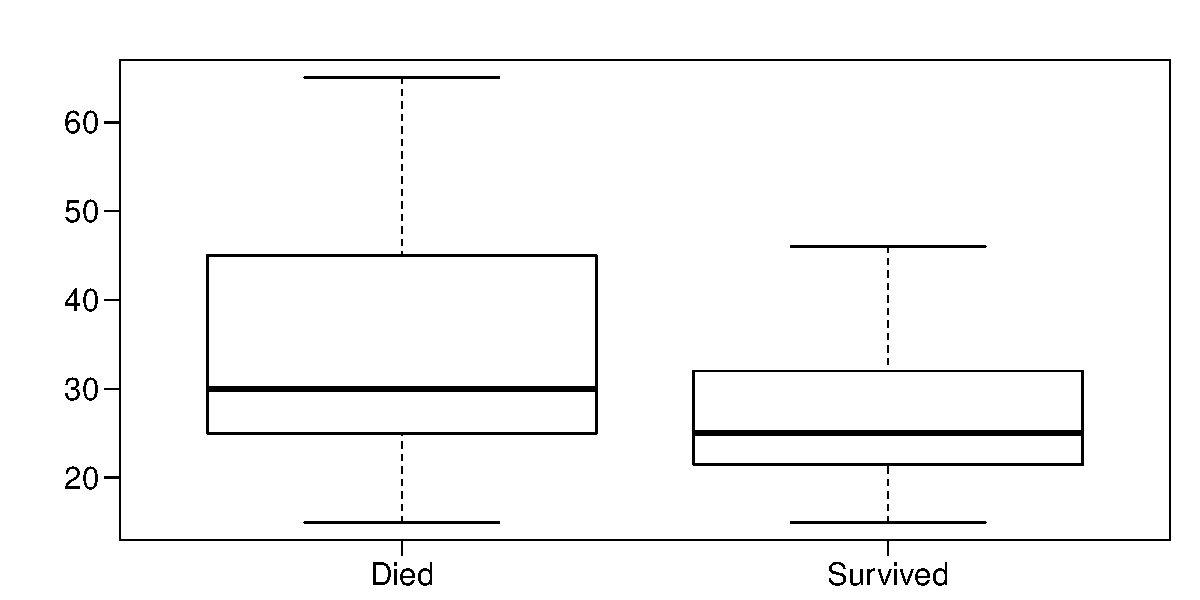
\includegraphics[width=0.82\textwidth]{figures/status_age.pdf}
\end{center}
\end{column}
\end{columns}

\end{frame}
%%%%%%%%%%%%%%%%%%%%%%%%%%%%%%%%%%%%%%%%%%%%%%%%%%%%%%%%%%%%%%%%%%%%%%%%
\begin{frame}{Activity 1}
\activity[-- binary response and success coding]{%
\textbf{Worksheet Part 1:} for each scenario, identify the binary response and state its success coding ($1=$ what?).}
\end{frame}
%%%%%%%%%%%%%%%%%%%%%%%%%%%%%%%%%%%%%%%%%%%%%%%%%%%%%%%%%%%%%%%%%%%%%%%%
\begin{frame}
\frametitle{Why not just fit a line?}
\examplehead{Donner Party}

Survival ($0$ or $1$) against age: every point sits on one of two rows.

\vspace{-0.3em}
\begin{center}
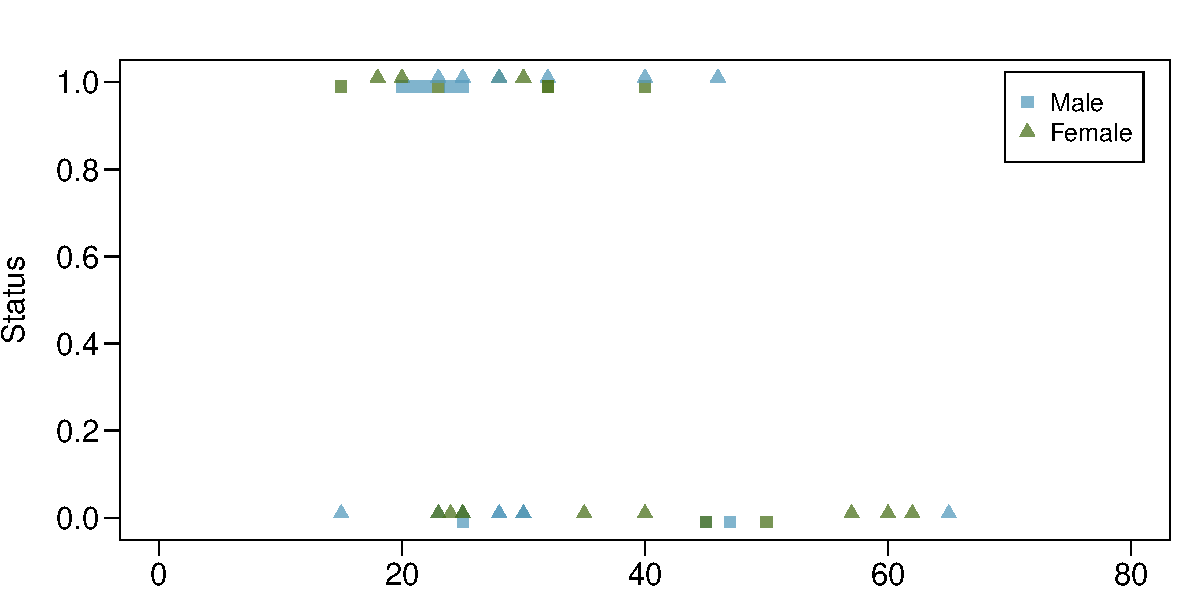
\includegraphics[width=0.42\textwidth]{figures/donner_scatter.pdf}
\end{center}

\vspace{-0.7em}
\textbf{What would a straight line through these points predict at age $70$?}

\pause
\vspace{-0.3em}
\caution{A line is unbounded: it predicts ``probabilities'' below $0$ and above $1$. We need a model that bends to stay inside $[0,1]$.}

\end{frame}
%%%%%%%%%%%%%%%%%%%%%%%%%%%%%%%%%%%%%%%%%%%%%%%%%%%%%%%%%%%%%%%%%%%%%%%%
\section{The logistic model}
%%%%%%%%%%%%%%%%%%%%%%%%%%%%%%%%%%%%%%%%%%%%%%%%%%%%%%%%%%%%%%%%%%%%%%%%
\begin{frame}
\frametitle{Building the model in two steps}

\textbf{Step 1 --- a linear predictor.} Exactly as in multiple regression, combine the predictors:
$$
\eta_i=\beta_0+\beta_1x_{i1}+\cdots+\beta_px_{ip},
\qquad\text{e.g.}\qquad
\eta_i=\beta_0+\beta_1\text{Age}_i+\beta_2\text{Female}_i.
$$
\vspace{0.2em}
\textbf{Step 2 --- squash it into a probability.} $\eta_i$ can be any real number, so pass it through the \hl{logistic function}:

\formula{Logistic regression}{%
\[
p_i=\text{logistic}(\eta_i)=\frac{e^{\eta_i}}{1+e^{\eta_i}}=\frac{1}{1+e^{-\eta_i}},
\qquad Y_i\sim\text{Bernoulli}(p_i).
\]}

\end{frame}
%%%%%%%%%%%%%%%%%%%%%%%%%%%%%%%%%%%%%%%%%%%%%%%%%%%%%%%%%%%%%%%%%%%%%%%%
\begin{frame}
\frametitle{The logistic function}

It maps \emph{any} real number to a probability between $0$ and $1$:

\begin{center}
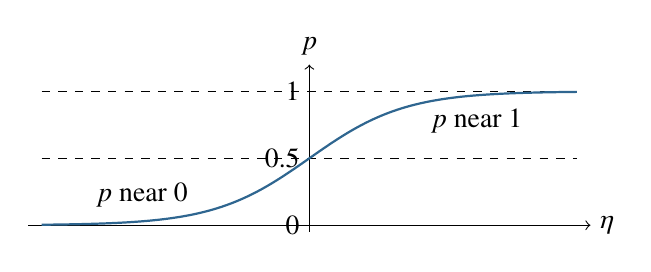
\begin{tikzpicture}[scale=0.85]
\draw[->] (-4.2,0) -- (4.2,0) node[right] {$\eta$};
\draw[->] (0,-0.1) -- (0,2.4) node[above] {$p$};
\draw[dashed] (-4,2) -- (4,2);
\draw[dashed] (-4,1) -- (4,1);
\node[left] at (0,2) {$1$};
\node[left] at (0,1) {$0.5$};
\node[left] at (0,0) {$0$};
\draw[thick,oiB,domain=-4:4,samples=120] plot (\x,{2/(1+exp(-1.4*\x))});
\node at (2.5,1.55) {$p$ near 1};
\node at (-2.5,0.45) {$p$ near 0};
\end{tikzpicture}
\end{center}

\vspace{-0.3em}
\begin{itemize}
\item $\eta=0 \Rightarrow p=0.5$; large positive $\eta \Rightarrow p$ near $1$; large negative $\eta \Rightarrow p$ near $0$.
\item The curve never reaches $0$ or $1$, so predictions stay legal.
\end{itemize}

\end{frame}
%%%%%%%%%%%%%%%%%%%%%%%%%%%%%%%%%%%%%%%%%%%%%%%%%%%%%%%%%%%%%%%%%%%%%%%%
\section{Odds and log odds}
%%%%%%%%%%%%%%%%%%%%%%%%%%%%%%%%%%%%%%%%%%%%%%%%%%%%%%%%%%%%%%%%%%%%%%%%
\begin{frame}
\frametitle{Probability, odds, and log odds}

\formula{Odds}{%
\[
\text{odds}=\frac{p}{1-p},
\qquad
\text{log odds}=\log\!\left(\frac{p}{1-p}\right).
\]}

\begin{itemize}
\item $p=0.50 \Rightarrow$ odds $=1$ (a fair bet).
\item $p=0.75 \Rightarrow$ odds $=3$ (success is 3 times as likely as failure).
\item $p=0.20 \Rightarrow$ odds $=0.25$.
\end{itemize}

Probabilities live in $[0,1]$; odds live in $[0,\infty)$; \emph{log} odds run over all real numbers --- the same range as $\eta$.

\end{frame}
%%%%%%%%%%%%%%%%%%%%%%%%%%%%%%%%%%%%%%%%%%%%%%%%%%%%%%%%%%%%%%%%%%%%%%%%
\begin{frame}
\frametitle{Step-by-step: probability to odds}

Suppose the model predicts a survival probability of $p=0.75$.

\begin{enumerate}
\item Probability of failure: \; $1-p=1-0.75=0.25$.
\pause
\item Odds of survival: \; $\text{odds}=\dfrac{p}{1-p}=\dfrac{0.75}{0.25}=3$.
\pause
\item Log odds: \; $\log(\text{odds})=\log(3)=1.10$.
\pause
\item Interpret in context:
\end{enumerate}

\pause
\vspace{-0.3em}
\workedexample[odds of 3]{Odds of $3$ mean survival is predicted to be \emph{three times as likely} as death, not that the probability is $3$.}

\end{frame}
%%%%%%%%%%%%%%%%%%%%%%%%%%%%%%%%%%%%%%%%%%%%%%%%%%%%%%%%%%%%%%%%%%%%%%%%
\begin{frame}
\frametitle{Logistic regression is linear in the log odds}

Rearranging $p=\dfrac{e^{\eta}}{1+e^{\eta}}$ gives the model in its most useful form:

\keyidea[-- The logit link]{%
\[
\log\!\left(\frac{p_i}{1-p_i}\right)=\eta_i=\beta_0+\beta_1x_{i1}+\cdots+\beta_px_{ip}.
\]
The model is a \emph{straight line} --- not in $p$, but in the \hl{log odds} of success.}

So a coefficient $\beta_j$ is a change in \emph{log odds}, not a change in probability. That is awkward to read directly, which is why we exponentiate.

\end{frame}
%%%%%%%%%%%%%%%%%%%%%%%%%%%%%%%%%%%%%%%%%%%%%%%%%%%%%%%%%%%%%%%%%%%%%%%%
\begin{frame}
\frametitle{Slope coefficients are odds ratios}

Since $\text{odds}=e^{\eta}$, increase $x_j$ by one unit, holding the others fixed:

\begin{itemize}
\item $\eta \longrightarrow \eta+\beta_j$
\pause
\item odds before: $e^{\eta}$ \qquad odds after: $e^{\eta+\beta_j}=e^{\eta}\,e^{\beta_j}$
\pause
\item so the odds get \emph{multiplied} by $e^{\beta_j}$:
\end{itemize}

\keyidea[-- Odds ratio]{%
\[
\frac{\text{odds after}}{\text{odds before}}=e^{\beta_j}.
\]
A one-unit increase in $x_j$ multiplies the odds of success by $e^{\beta_j}$, holding the other predictors fixed. For a change of $\Delta$ units, the odds are multiplied by $e^{\beta_j\Delta}$.}

\end{frame}
%%%%%%%%%%%%%%%%%%%%%%%%%%%%%%%%%%%%%%%%%%%%%%%%%%%%%%%%%%%%%%%%%%%%%%%%
\begin{frame}
\frametitle{Activity 2}

\activity[-- converting between scales]{%
\textbf{Worksheet Part 2.}
Fill in the missing values.

\begin{center}
\begin{tabular}{c c c}
\toprule
$p$ & odds & log odds \\
\midrule
0.50 & & \\
0.80 & & \\
0.25 & & \\
\bottomrule
\end{tabular}
\end{center}}

\pause
\soln{$0.50$: odds $=1$, log odds $=0$. \quad $0.80$: odds $=4$, log odds $=\log 4\approx1.386$. \quad $0.25$: odds $=1/3$, log odds $=\log(1/3)\approx-1.099$.}

\end{frame}
%%%%%%%%%%%%%%%%%%%%%%%%%%%%%%%%%%%%%%%%%%%%%%%%%%%%%%%%%%%%%%%%%%%%%%%%
\section{Fitting by maximum likelihood}
%%%%%%%%%%%%%%%%%%%%%%%%%%%%%%%%%%%%%%%%%%%%%%%%%%%%%%%%%%%%%%%%%%%%%%%%
\begin{frame}
\frametitle{How is logistic regression fit?}

Least squares does not apply: the response is $0/1$, and we are modeling a \emph{probability}. Instead we use \hl{maximum likelihood}, the same recipe as Lecture 2:

\begin{enumerate}
\item Write down a probability model.
\item Write down its likelihood.
\item Choose the parameter values that maximize it.
\end{enumerate}

\keyidea{Choose the curve that makes the observed $0$s and $1$s most plausible: survivors get high predicted probabilities, non-survivors low ones.}

\end{frame}
%%%%%%%%%%%%%%%%%%%%%%%%%%%%%%%%%%%%%%%%%%%%%%%%%%%%%%%%%%%%%%%%%%%%%%%%
\begin{frame}
\frametitle{The Bernoulli likelihood}

For a single observation, $Y_i\sim\text{Bernoulli}(p_i)$, so
$$
P(Y_i=y_i)=p_i^{\,y_i}(1-p_i)^{1-y_i}
\qquad
\begin{cases}
=p_i, & \text{if } y_i=1,\\[2pt]
=1-p_i, & \text{if } y_i=0.
\end{cases}
$$
\pause
Assuming the observations are independent, multiply them together:

\formula{Likelihood}{%
\[
L(\beta)=\prod_{i=1}^n p_i^{\,y_i}(1-p_i)^{1-y_i},
\qquad
p_i=\frac{e^{\beta_0+\beta_1x_{i1}+\cdots+\beta_px_{ip}}}{1+e^{\beta_0+\beta_1x_{i1}+\cdots+\beta_px_{ip}}}.
\]}

Unlike least squares, there is no closed-form solution, so software maximizes it numerically.

\end{frame}
%%%%%%%%%%%%%%%%%%%%%%%%%%%%%%%%%%%%%%%%%%%%%%%%%%%%%%%%%%%%%%%%%%%%%%%%
\section{Interpreting the fitted model}
%%%%%%%%%%%%%%%%%%%%%%%%%%%%%%%%%%%%%%%%%%%%%%%%%%%%%%%%%%%%%%%%%%%%%%%%
\begin{frame}
\frametitle{Model 1: age only}
\examplehead{Donner Party}

Fitting \texttt{glm(Status $\sim$ Age, family = binomial)} gives
$$
\log\!\left(\frac{p}{1-p}\right)=1.8185-0.0665(\text{Age}).
$$
\vspace{-0.4em}
\begin{center}
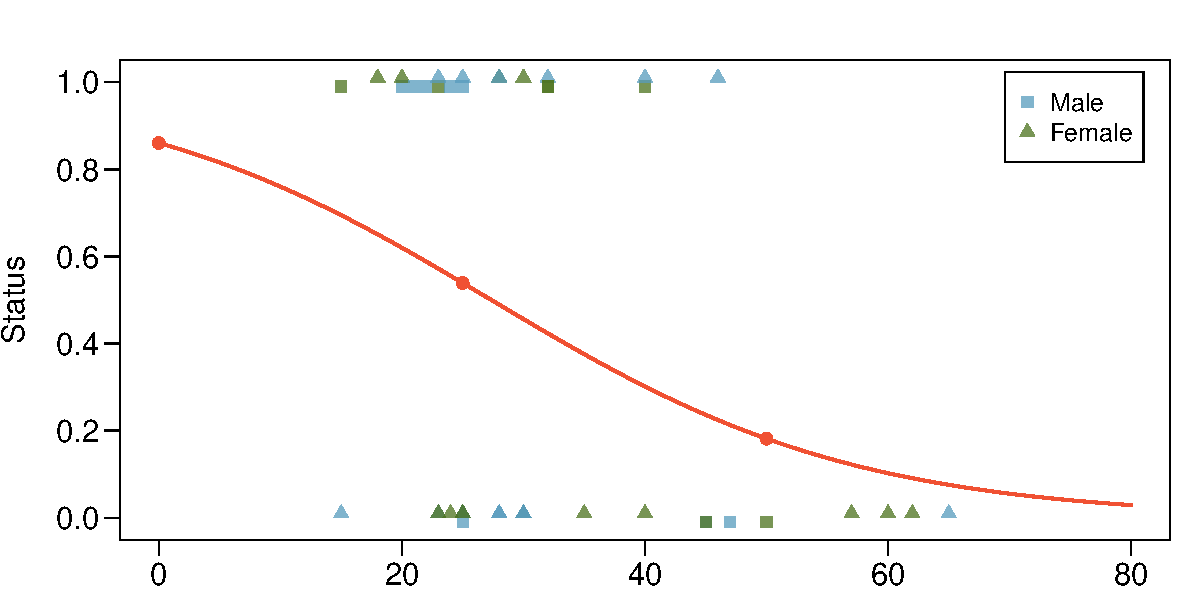
\includegraphics[width=0.48\textwidth]{figures/donner_scatter_pred.pdf}
\end{center}

\vspace{-0.5em}
The fitted curve bends: survival probability falls smoothly with age, but never leaves $[0,1]$.

\end{frame}
%%%%%%%%%%%%%%%%%%%%%%%%%%%%%%%%%%%%%%%%%%%%%%%%%%%%%%%%%%%%%%%%%%%%%%%%
\begin{frame}
\frametitle{Model 2: age and sex}

\examplehead{Donner Party}

Sex is categorical, so it enters through a $0/1$ indicator (as in Lecture 5), with \hl{Male as the reference level}.

{\small
\begin{center}
\begin{tabular}{l r r r}
\toprule
Term & Estimate & Std. Error & $p$-value \\
\midrule
(Intercept) & 1.6331 & 1.1102 & 0.1413 \\
Age & $-0.0782$ & 0.0373 & 0.0359 \\
SexFemale & 1.5973 & 0.7555 & 0.0345 \\
\bottomrule
\end{tabular}
\end{center}}

\pause
$$
\log\!\left(\frac{p}{1-p}\right)=1.6331-0.0782(\text{Age})+1.5973(\text{Female}).
$$
\end{frame}
%%%%%%%%%%%%%%%%%%%%%%%%%%%%%%%%%%%%%%%%%%%%%%%%%%%%%%%%%%%%%%%%%%%%%%%%
\begin{frame}
\frametitle{Visualizing the model: two curves}
\examplehead{Donner Party}

\begin{center}
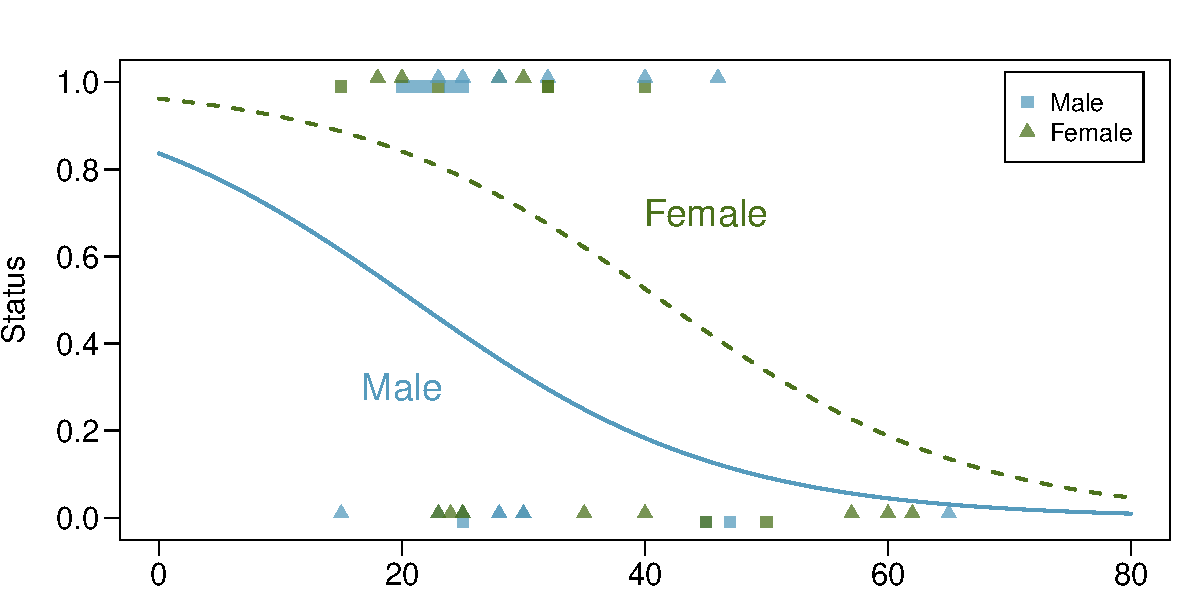
\includegraphics[width=0.66\textwidth]{figures/donner_scatter_both.pdf}
\end{center}

\vspace{-0.6em}
\keyidea[-- The indicator shifts the curve]{Just as an indicator gave us \emph{parallel lines} in Lecture 5, here it gives two \emph{parallel logistic curves} --- same shape, shifted. At every age, the female curve sits above the male one.}

\end{frame}
%%%%%%%%%%%%%%%%%%%%%%%%%%%%%%%%%%%%%%%%%%%%%%%%%%%%%%%%%%%%%%%%%%%%%%%%
\begin{frame}
\frametitle{Step-by-step: age as an odds ratio}
\examplehead{Donner Party}

The age coefficient is $-0.0782$.

\begin{enumerate}
\item A coefficient is a change in \hl{log odds}: one extra year shifts the log odds of survival by $-0.0782$.
\pause
\item Exponentiate to turn it into an \hl{odds ratio}: \; $e^{-0.0782}=0.925$.
\pause
\item Interpret in context:
\end{enumerate}

\pause
\workedexample[age]{Holding sex fixed, each additional year of age \emph{multiplies} the odds of survival by about $0.925$: a $7.5\%$ drop per year. Over $10$ years the odds are multiplied by $e^{-0.0782\times 10}=0.458$, cutting them roughly in half.}

\end{frame}
%%%%%%%%%%%%%%%%%%%%%%%%%%%%%%%%%%%%%%%%%%%%%%%%%%%%%%%%%%%%%%%%%%%%%%%%
\begin{frame}
\frametitle{Step-by-step: sex as an odds ratio}
\examplehead{Donner Party}

The \texttt{Female} coefficient is $1.5973$ (reference level: Male).

\begin{enumerate}\setlength{\itemsep}{2pt}
\item Being female shifts the \hl{log odds} of survival by $+1.5973$.
\pause
\item Exponentiate: \; $e^{1.5973}=4.94$.
\pause
\item Interpret in context:
\end{enumerate}

\pause
\vspace{-0.5em}
\workedexample[sex]{Holding age fixed, women had about $4.94$ times the \emph{odds} of survival that men of the same age did.}

\pause
\vspace{-0.5em}
\caution{An odds ratio is \emph{not} a ratio of probabilities: ``$4.94\times$ the odds'' $\neq$ ``$4.94\times$ as likely''.}

\end{frame}
%%%%%%%%%%%%%%%%%%%%%%%%%%%%%%%%%%%%%%%%%%%%%%%%%%%%%%%%%%%%%%%%%%%%%%%%
\begin{frame}
\frametitle{Prediction: from log odds back to probability}
\examplehead{Donner Party}

For a $25$-year-old man, set $\text{Age}=25$ and $\text{Female}=0$:
\begin{align*}
\eta &= 1.6331-0.0782(25)+1.5973(0) = -0.322,\\
\pause
p &= \frac{e^{\eta}}{1+e^{\eta}} = \frac{e^{-0.322}}{1+e^{-0.322}} = 0.420.
\end{align*}
\pause
The model puts his probability of survival at about \hl{$42\%$} --- note this is a \emph{probability}, not an odds.

\end{frame}
%%%%%%%%%%%%%%%%%%%%%%%%%%%%%%%%%%%%%%%%%%%%%%%%%%%%%%%%%%%%%%%%%%%%%%%%
\begin{frame}
\frametitle{Activity 3}

\activity[-- interpret an odds ratio]{%
\textbf{Worksheet Part 3.}
A logistic regression model predicts whether an email is spam:
\[
\log\!\left(\frac{p}{1-p}\right)=-3.2+0.45(\text{num\_links}).
\]
Interpret the coefficient $0.45$ as an odds ratio.}

\pause
\solnbox{$e^{0.45}=1.57$. Each additional link multiplies the odds that the email is spam by about $1.57$: a $57\%$ increase in the odds per link.}

\end{frame}
%%%%%%%%%%%%%%%%%%%%%%%%%%%%%%%%%%%%%%%%%%%%%%%%%%%%%%%%%%%%%%%%%%%%%%%%
\section{Classification and unbalanced data}
%%%%%%%%%%%%%%%%%%%%%%%%%%%%%%%%%%%%%%%%%%%%%%%%%%%%%%%%%%%%%%%%%%%%%%%%
\begin{frame}
\frametitle{From a probability to a decision}

The model returns a \emph{probability}, $\widehat{p}=P(Y=1\mid x)$. But acting on it requires a \emph{label} --- spam or not, treat or not.

\vspace{0.4em}
To label, pick a \hl{threshold}:
$$
\widehat{p}\ge c \quad\Longrightarrow\quad \widehat{Y}=1.
$$
\pause
\dq{Should the threshold always be $c=0.50$?}

\pause
\soln{No. The rest of this section is about why. The model estimates probabilities; the threshold is a separate \emph{decision}.}

\end{frame}
%%%%%%%%%%%%%%%%%%%%%%%%%%%%%%%%%%%%%%%%%%%%%%%%%%%%%%%%%%%%%%%%%%%%%%%%
\begin{frame}
\frametitle{Two ways to be wrong}

Once we label, every observation falls into one of four cells:

\begin{center}
\begin{tabular}{l c c}
\toprule
 & Actual 1 & Actual 0 \\
\midrule
Predicted 1 & true positive (TP) & \hl{false positive (FP)} \\
Predicted 0 & \hl{false negative (FN)} & true negative (TN) \\
\bottomrule
\end{tabular}
\end{center}

\vspace{0.5em}
\begin{itemize}
\item \textbf{False positive:} we cried wolf --- predicted success, but it failed.
\item \textbf{False negative:} we missed it --- predicted failure, but it succeeded.
\end{itemize}

The threshold decides how these two errors are traded off against each other.

\end{frame}
%%%%%%%%%%%%%%%%%%%%%%%%%%%%%%%%%%%%%%%%%%%%%%%%%%%%%%%%%%%%%%%%%%%%%%%%
\begin{frame}
\frametitle{Activity 4}

\activity[-- classify with threshold $0.50$]{%
\textbf{Worksheet Part 4.}
A spam model gives these predicted probabilities.

{\small
\begin{center}
\begin{tabular}{c c c c c c c c}
\toprule
Email & 1 & 2 & 3 & 4 & 5 & 6 & 7 \\
\midrule
$\widehat{p}$ & .92 & .81 & .63 & .48 & .33 & .21 & .08 \\
Actual & 1 & 0 & 1 & 1 & 0 & 0 & 0 \\
\bottomrule
\end{tabular}
\end{center}}

Using $c=0.50$, classify each email and count TP, FP, TN, FN.}

\pause
\solnbox{Predicted spam: emails 1, 2, 3. \quad TP $=2$, \; FP $=1$, \; TN $=3$, \; FN $=1$.}

\end{frame}
%%%%%%%%%%%%%%%%%%%%%%%%%%%%%%%%%%%%%%%%%%%%%%%%%%%%%%%%%%%%%%%%%%%%%%%%
\begin{frame}
\frametitle{Activity 5}

\activity[-- now raise the threshold to $0.75$]{%
Same emails, stricter rule: $c=0.75$.

{\small
\begin{center}
\begin{tabular}{c c c c c c c c}
\toprule
Email & 1 & 2 & 3 & 4 & 5 & 6 & 7 \\
\midrule
$\widehat{p}$ & .92 & .81 & .63 & .48 & .33 & .21 & .08 \\
Actual & 1 & 0 & 1 & 1 & 0 & 0 & 0 \\
\bottomrule
\end{tabular}
\end{center}}

Re-classify and count. What changed, and what did it cost?}

\pause
\solnbox{Predicted spam: emails 1, 2. \quad TP $=1$, \; FP $=1$, \; TN $=3$, \; FN $=2$. \; Raising the bar did \emph{not} remove the false positive, but it cost a true positive: one more real spam slipped through.}

\end{frame}
%%%%%%%%%%%%%%%%%%%%%%%%%%%%%%%%%%%%%%%%%%%%%%%%%%%%%%%%%%%%%%%%%%%%%%%%
\begin{frame}
\frametitle{The threshold tradeoff}

\begin{center}
\begin{tabular}{l c l}
\toprule
\textbf{Lower the threshold} & & \textbf{Raise the threshold} \\
\midrule
label more cases as $1$ &  &label fewer cases as $1$ \\
catch more true positives & & miss more true positives \\
\hl{get more false positives} & & \hl{get fewer false positives} \\
\bottomrule
\end{tabular}
\end{center}

\vspace{0.5em}
\keyidea[-- No free lunch]{You cannot reduce both errors at once by moving the threshold. Moving it trades false positives against false negatives --- so the right threshold depends on which error is more costly.}

\end{frame}
%%%%%%%%%%%%%%%%%%%%%%%%%%%%%%%%%%%%%%%%%%%%%%%%%%%%%%%%%%%%%%%%%%%%%%%%
\begin{frame}
\frametitle{Measuring performance: accuracy}

\formula{Accuracy}{%
\[ \text{accuracy}=\frac{\#\text{ correct predictions}}{n}=\frac{TP+TN}{n}. \]}

For the email activity at threshold $0.50$: accuracy $=(2+3)/7\approx 71\%$.

\dq{Is high accuracy always good news?}
\end{frame}
%%%%%%%%%%%%%%%%%%%%%%%%%%%%%%%%%%%%%%%%%%%%%%%%%%%%%%%%%%%%%%%%%%%%%%%%
\begin{frame}
\frametitle{Unbalanced data: when accuracy is misleading}

A binary outcome is \hl{unbalanced} when one class is far more common. Of $1000$ emails only $50$ are spam. Suppose a ``classifier'' labels \emph{every} email as not spam:

{\footnotesize
\begin{center}
\begin{tabular}{lcc}
\toprule
 & Actual not spam & Actual spam \\
\midrule
Predicted not spam & 950 & 50 \\
Predicted spam & 0 & 0 \\
\bottomrule
\end{tabular}
\end{center}}

\vspace{-0.3em}
\textbf{What is its accuracy? What is the problem?}

\pause
\vspace{-0.2em}
\caution{Accuracy is $950/1000=95\%$, yet it catches \emph{none} of the 50 spam emails. On unbalanced data, high accuracy can come from ignoring the rare class --- the class we care about.}

\end{frame}
%%%%%%%%%%%%%%%%%%%%%%%%%%%%%%%%%%%%%%%%%%%%%%%%%%%%%%%%%%%%%%%%%%%%%%%%
\begin{frame}{Activity 6}
\activity[-- misleading accuracy]{%
\textbf{Worksheet Part 5:} for an unbalanced testing scenario, compute the accuracy of a trivial classifier and explain why it is misleading.}
\end{frame}
%%%%%%%%%%%%%%%%%%%%%%%%%%%%%%%%%%%%%%%%%%%%%%%%%%%%%%%%%%%%%%%%%%%%%%%%
\begin{frame}
\frametitle{Choosing a threshold is a decision problem}

\begin{itemize}
\item \textbf{Disease screening:} a false negative sends a sick patient home. Lower the threshold.
\item \textbf{Spam filtering:} a false positive buries an important email in the junk folder. Raise it.
\item \textbf{Fraud detection:} the class of interest is rare, so accuracy is the wrong yardstick entirely.
\end{itemize}

\vspace{0.6em}
\keyidea[-- Model vs.\ decision]{The statistical model estimates probabilities. The threshold turns probabilities into \emph{actions} --- and that step needs the costs of the two errors, which statistics alone cannot supply.}

\end{frame}
%%%%%%%%%%%%%%%%%%%%%%%%%%%%%%%%%%%%%%%%%%%%%%%%%%%%%%%%%%%%%%%%%%%%%%%%
\section{Wrap-up}
%%%%%%%%%%%%%%%%%%%%%%%%%%%%%%%%%%%%%%%%%%%%%%%%%%%%%%%%%%%%%%%%%%%%%%%%
\begin{frame}
\frametitle{Key takeaways}

\begin{itemize}
\item Code the binary response so that success $=1$, and model $Y\sim\text{Bernoulli}(p)$.
\item Build $\eta=\beta_0+\beta_1x_1+\cdots$, then squash it: $p=e^{\eta}/(1+e^{\eta})$.
\item Read the model on the \hl{log odds} scale, where it is linear.
\item Exponentiate a coefficient to get an \hl{odds ratio}: $e^{\beta_j}$.
\item Fit by \hl{maximum likelihood}, not least squares.
\item To classify, choose a threshold; on unbalanced data, never trust accuracy alone.
\end{itemize}

\end{frame}
%%%%%%%%%%%%%%%%%%%%%%%%%%%%%%%%%%%%%%%%%%%%%%%%%%%%%%%%%%%%%%%%%%%%%%%%

%%%%%%%%%%%%%%%%%%%%%%%%%%%%%%%%%%%%
% End document
%%%%%%%%%%%%%%%%%%%%%%%%%%%%%%%%%%%%

\end{document}
